\documentclass[11pt]{article}
\usepackage{graphicx}
\usepackage{hyperref}
\usepackage{fancyhdr}
\usepackage{setspace}
\pagestyle{fancy}
\fancyhead{}
\fancyfoot{}
\fancyfoot[C]{-\thepage-}
\fancyfoot[L]{ID:997900158}
\fancyfoot[RO]{MPM406 - Random Clinical Trial}
\renewcommand{\footrulewidth}{0.4 pt}
\renewcommand{\headrulewidth}{0 pt}

\hypersetup{colorlinks = true, linkcolor = blue, citecolor = blue}
\title{Two Factorial Randomized Clinical Trial comparing dose and timing of estrogen supplementation on the prevention of athersclerotic cardiovascular disease in post menopausal women}
\author{Student ID: 997900158}
\date{\today}
\begin{document}
	\maketitle
	\begin{abstract}
		This two factorial multicenter randomized clinical trial was conducted on a convenience sample of peri-menopausal women presenting to North American Kaiser Permanente hospitals in 2001-2002.
		The women were given differing levels of estrogen supplementation both before and after the onset of menopause, and the level of carotid inter-media thickness measured to assess progression of athersclerotic cardiovascular disease, as well as cases of clincial athersclerotic cardiovascular disease recorded.
		The women were followed up for 8 years (until 2010) results revealed early supplementation of low dose estrogen is as protective as high dose, but with less side effects.

	\end{abstract}

\onehalfspace
	\section{Introduction} 
		Athersclerotic cardiovascular disease is an important cause of cardiovascular dissease in post-menopausal women.
		In 1994, Cardiovascular disease killed a half million women and accounted for over 40\% of all deaths in women, more than all forms of cancer combined\cite{AHA1997}.
		Even though there has been an overall decline in the death rate due to cardiovascular disease in the United States over several decades, the rate of decline is less for women and especially african-american women \cite{Mosca1997}.
		While men are more commonly affected by cardiovascular disease, risk increases rabpidly in women as they age, doubles every decade after age 55\cite{Gordon1978}. 
		It has been shown that reduced circulating ostradiol during menopause increases atherogenic lipids and reduces carotid blood flow, causing increased incidence of athersclerotic cardiovascular disease \cite{Hodis}.
		Menopause is the abcence of a menstural cycle in the previous 12 months, and occurs at an average age of 51 but can range between 45 and 55 years \cite{Gold2012}. 
		Supplamental oestrogen has been used for some time to treat symptoms of menopause and its associated increase in athersclerotic cardiovascular disease risk, however serious side effects ( higher risk of breast cancer, increased blood clots and endometrial cancer) have been documented \cite{Gold2012}.
		Recent research has also questioned the cardiovascular protection associated with menopausal hormonal therapy and concluded no overall benfit to supplamental estrogen overall, and a possible interaction between time of therapy initiation and protection provided \cite{Anderson2004,Prentice2009}.
		Since the initial reasearch questioning the efficacy of menopausal hormonal therapy was completed, there have been numerous innovations in the form and dose of estrogen deliverey have occurred, and it is hypothesised that these new forms/dosing regiemes may provide improved protention.



		This two-by-two factorial radomized clinical trial is designed to assess the effects of intiating estradiol supplementation at diffent doses and different times following the onset of menopause on the risk of athersclerotic cardiovascular disease.
		The study Hypothesis is that initiating estrogen therapy before the onset of menopause is protective of athersclerotic cardiovascular disease, and that a reduced dose of estrogen provides the same protection with reduced side effects.


	\section{Methods} 
		The study population was drawn from women presenting to Kaiser Permanente between 2000-01-01 and 2009-12-31, between the ages of 40 and 50 that were undergoing signs of peri-menopause (last cycle less than 12 months ago, but no regular monthly cycle).
		Kaiser Permanente is a managed care consortium based in northern California. It has almost 15,000 physicians operating in 650 facilities spread over 9 states, and serves nearly 9 million members \cite{Rauber}.
		On identifying a possible study subject, a full physical examination and medical history was taken, and where possible validated with a central database of historical medical records maintained by Kaiser Permanente.
		During this physical examination BP, BMI, race, and age were measured, and lifdestyle factors such as smoking and phjysical activity levels recorded.
		Blood was also collected during this initial examination and levels of lipoprotiens measured.
		Any woman with a previous hysterectomy, had taken estrogen suppleaments in the past, or had experienced any prolonged angina was disqualified from the study as hysterectomy causes instant menopause at any age, and angina may be a sign of preexisting heart conditions.
		

		Sample size recquirements were calculated using epi-info with a subclinical athersclerotic cardiovascular disease rate of 25\%
		Interim analysis were completed at bi-yearly intervals by an independent data and safety monitoring comitee, and the decision to procedd based on participant safetey (no increased rates of side effects or athersclerotic cardiovascular disease) and the percieved benefit of continuing with study.
		O’Brien-Flemming spending strategy was used to generate stopping boundaries for each planned analysis.


		Two factorial design was chosen to allow simountaneus comparison of dose and timing effects, and the use of a very large sample size allowed the assessment of interactions at sufficeint power. 
		The two dose levels chosen were 0.625mg and 0.3mg of conjugated equine estrogens, delivered per os.
		0.625 mg SID PO is the standard therapy currently in use, the lower dose of 0.3mg has been suggested as a way to maximise benefit ( menopause symptoms, CVD,osteoporosis), while minimising harmful side effects (cancer risk, blood clots)  associated with estrogen.
		The two timing levels chosen were initiation of therapy during peri menopause, or initiation 3 years after menopause.
		The use of a two factorial design resulted in 4 study groups, as described in \hyperref[Figure 1]{figure1}.


		Patients were randomised using a centralised allocation procedure, with both patient and physician blinded to allocation method. 
		After eligibility was established, an auto generated email containing patient information was sent to a server maintained in the researchers office at Kaiser Permanente's headquarters in Oakland, California. 
		This computer used a schedule of random numners generated from open radio freqency atmoshperic noise \cite{Eddelbuettel2009}  and study participants were allocated to one of the four groups basd on this number.
		The allocation, general patient details, and source and timsetamp of the allocation request were recorded and compared to doctors own records of assignment to ensure accuracy.
		The result of this allocation was returned to the physician in an email with a number 1-4 and the appropriate treatment initiated.


		Following assignment, all patients recieved a 6 month supply of pills, regardless of group assignment.
		This pill pack was in nondescript packaging, with only a number label, and was renewed every 6 months by mail from Kaiser Permanente headquarters.
		Even after assignment, the sequence and allocation was concealed from study participant and physician.
		Those that were assigned late deliverey of either dose were initially given sugar pills that had same appearance, taste, and smell as the real estrogen pills. 
		3 years after menopause was determined to have taken place ( more than 12 months amenorrhoea) had their next 6 monthly supply of pills converted to estrogen, at a dose depending on their assignement. Again there was no way to tell the difference between pills having different doses.

		
		Patients had annual checkups with their Kaiser Permanente physician during the study period.
		During this examination, a standard examination and history was performed, as well specific questions relating to the onset of menopause, symptoms experienced during the year, and any incidence of angina or clinical cardiovascular disease.
		Side effects of estrogen therapy monitored included cancer (breast, colon, endometrial), and clotting events (Deep Vein Thrombosis, Ischaemic stroke)
		All women had their responses checked against actual medical history, improving accuracy of data and minimising recall bias.
		To assess the progression of subclinical athersclerotic cardiovascular disease, women had a carotid ultrasound to measure carotid arterey intima-media thickness.
		The thickness of carotid arterey intima-media was recorded and compared to previous measurements to assess disease progression.
		This intervention was well tolerated as women were presenting to their health professional for an annual checkup anyway, and the Carotid ultrasound is quick and non-invasive
		In addition, the quality of these measurments were maintained by using a trained ultrasonographer at each of the Kaiser Permanente facilities.
		Before the beginnning of enrollment, these ultrasonographers were trained at a central location on a standard protocol for taking measurements, and the inter-observer agreement assessed by completing an examination of 5 test subjects.


		All patients were thoroughly briefed on the study design and interventions, and signed informed consent and liability release forms.


	\subsection{Statistical Evaluation}
		The primary study endpoint was progression of subclinical athersclerotic cardiovascular disease defined as an increase in carotid inter-media thickness of more than 0.0035mm per year diagnosed on carotid ultrasound.
		A second study endpoint was clinical athersclerotic cardiovascular disease, which included stroke, congestive heart disease, and death due to cardiac causes.


		Kaplan-Meier survival curves for overall survival were compared by log-rank test, and the unadjusted HR (and 95\% CI) was calculated using a Cox regression analysis.
		As a secondary analysis, potential covariates (race, age, smoking, physical activity levels) were included in the Cox regression model to generate an adjusted HR for overall survival.



		All analysis was completed on an intention to treat basis, and all statistical analysis were completed in R \cite{RCoreTeam2012} on data that had a random hashing algorithm performed before analysis, ensuring blinding of statistitians.



	\section{Results}
		43,426 women were intially enrolled in this study, with 42,236 assigned to a treatment group and 38,234 completing and were analysed in the study (As shown in the \hyperref[Study Flow]{flow}
		Baseline characteristics of study participant can be seen in \hyperref[Table 1]{table1}.


		The incidence of side effects that can be caused by estrogen is shown in \hyperref[Table 2]{table2}, Comparison rates in post menopausal women not undergoing menopausal hormonal therapy are shown for comparison.
		As can be seen from table2, ther eis no increased risk of side effects associated with menopausal hormonal therapy.




		The compliance rate among study participants was assesed by measuring estrogen levels in blood of a sample (n=100) of participants recieving estrogen at least 2 years following menopause. Compliance was found to be good, at 93\%, and no adjustment was made for those found to be non compliant.

		
		The rates of diagnosis on each ultrasonographer were compared to ensure inter-observer agreement.
		As each ultrasonographer completed many measurements, each individual observer distribution was compared to the average distribution of all observers, to determine if any one observer was over or under measuring carotid inter-media thickness.
		The interobserver correlation was above 90\% and no single observer consistently over or under measured carotid inter-media thickness.
		The measuremnents between ultrasonographers were compared 


	\section{Discussion} 


	\subsection{Strengths and Limitations}
		Data quality was a strenth of this study.
		Cross validating the patients oral medical histories with the actual recorded histories from the Kaiser Permanente central databases ensures accuracy and reduces recall bias.
		Allocation of participants to study groups was entirely random and repeatable, and the comparison of allocation and actual treatment records allowed analysis to be undertaken on an accurate intention to treat basis. 


		The triple blinding methods used in this study were also a strength, with study participants, consulting physicians, and statistitians all unaware of which group participants/data were assigned to.


		A potential limitation of this study was the selection of study participants from Kaiser Permanente hopitals.
		Rates of insurance are correlated with Socio economic status and Education level, both factors that are also associated with use of menopausal hormonal therapy.
		There may be some relationship between lifestyle factors/SES and progression of athersclerotic cardiovascular disease, and out attemp to control for these factors (correcting for smoking and activity levels) may be insufficient.


		Another potential limitation is the loss of blinding to study participants based on the effects of treatment. Some women experience bleeding when taking an estrogen supplement, and this would remove blinding.
		
	\section{Figures}

\begin{figure*}[h!]
	\centering
	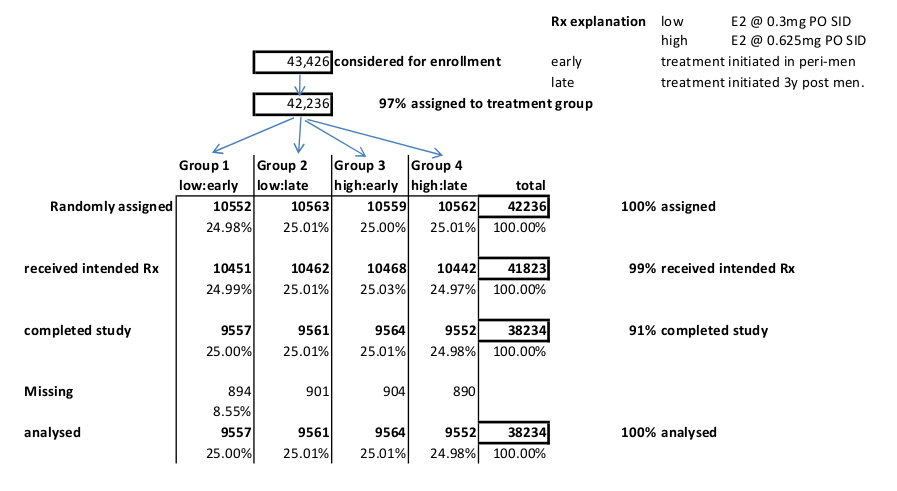
\includegraphics[scale=0.5]{figure1.jpg}
	\caption{Flow Diagram showing study participant allocation}
	\label{flow}
\end{figure*}

\begin{figure*}[h!]
	\centering
	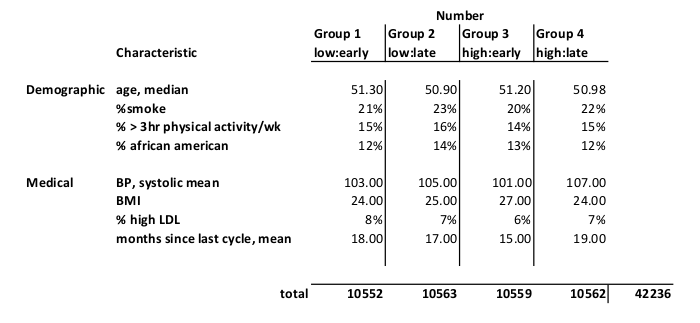
\includegraphics[scale=0.6]{table1.jpg}
	\caption{Characteristics of study participants.}
	\label{table1}
\end{figure*}
 
\begin{figure*}[h!]
	\centering
	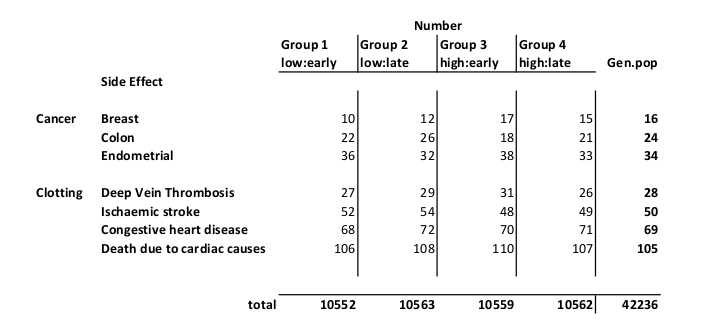
\includegraphics[scale=0.7]{table2.jpg}
	\caption{Incidence of Side effects in study groups}
	\label{table2}
\end{figure*}

\begin{figure*}[h!]
	\centering
	\includegraphics[scale=0.6]{sample.jpg}
	\caption{Sample size function and calculation output from R. Calculations agrees with Epi Info when continuity correction was applied.}
	\label{sample}
\end{figure*}

\clearpage
\bibliographystyle{unsrt}
\bibliography{wom}



\end{document}

%%%%%

% interactoins - 
%% make streamlined as possible. but need at least one confounder, not necc any interactions, can say did not find any (kim paper for technique - none stat sig so not included). potential effect modify - wualitative. 
% if include need to show OR with and without interactions.
% table 1 - cats in study,. throw in other factors that wont include - make them the same. e.g. age w exposure outcome and not on causal path. - no sig p value. 
% fig 1 - exposure b \emph{Bartonella sp.} , outcome ev.

% diagram bartonella causing uveitis, age associated w bartonella and uveitis (double ended arrow.) then show in table.( anythign in table that same do not need to have in diagram.
